\textbf{Quick Time Selection}

In this section, users can quickly set the desired time range for their data analysis. By using the time selection slider, users can adjust the range by simply moving the indicator along the timeline. This allows for a smooth and intuitive way to select specific periods for viewing data. The slider lets users choose from various predefined time frames, such as Last Hour, Last 24 Hours, and more.

\begin{figure}[h]
  \centering
  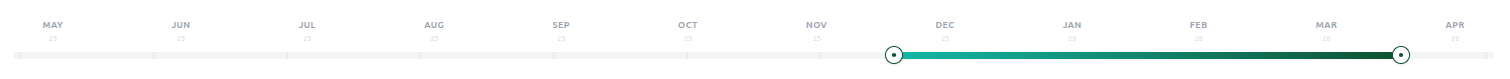
\includegraphics[width=\textwidth]{img/common/commonarea/QuickTimeSelection.png}
  \caption{Example of Quick Time Selection}
\end{figure}

As the user moves the slider, the time range is automatically updated, reflecting the selected period. This feature provides a dynamic and user-friendly interface for analyzing data across different time intervals.